\graphicspath{{Backgrounds/Figures/}}

\chapter{Backgrounds}

Backgrounds in particle physics experimental studies are processes that have similar final states to the process that is being studied. Because of their similar final states with the process of interest, background signal can be mistaken as the signal of the process being studied. That is why backgrounds are experimental noise that is not desirable in a study and that has to be eliminated as much as possible. In this particular study three backgrounds were considered because of their similarity in the final states with the one of the heavy neutrino production. 

One of the backgrounds considered for this analysis was the W + jets process shown in Figure \ref{fig: Wjets_background}. This process is considered as a background for the heavy neutrino production because of the presence of one lepton coming from the decay of the W boson in the process. It can be noted that in principle this process would not have the second lepton present in the heavy neutrino production process. However, it is has to be remembered that taus are observed as jets in the detector. There is a possibility of tagging a jet as a tau incorrectly. Since the gluon, the quark $b$ and the other quark present in the process are also observed in the detector as jets, these could by identified incorrectly as a tau. If one of these jets is tagged incorrectly, then the final state of the W + jets process would be the same as the one of the heavy neutrino process because it would be identified as a process with two leptons and two jets. 

\begin{figure}[H]
\centering
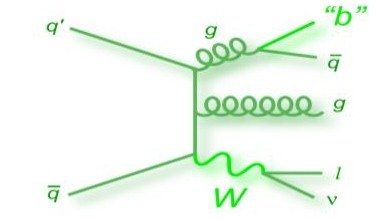
\includegraphics[width = 0.7\linewidth]{Wjets}
\caption{Feynman diagram of W+jets process}
\label{fig: Wjets_background}
\end{figure}

Another background considered was the $t\bar{t}$ semileptonic process that contains the decay of a gluon into the quarks top and anti-top as shown in Figure \ref{fig: ttbar_background}. As in the case of the W + jets process, the $t\bar{t}$ semileptonic background has only one lepton in its final state. However, as mentioned earlier, this process would be observed in the detector as two jets coming from the b quark, or B-jets, and two jets coming from the other two quarks. If one of the four is tagged incorrectly as a $\tau$, the final state would be identical to the one of the heavy neutrino process studied in the analysis.


\begin{figure}[H]
\centering
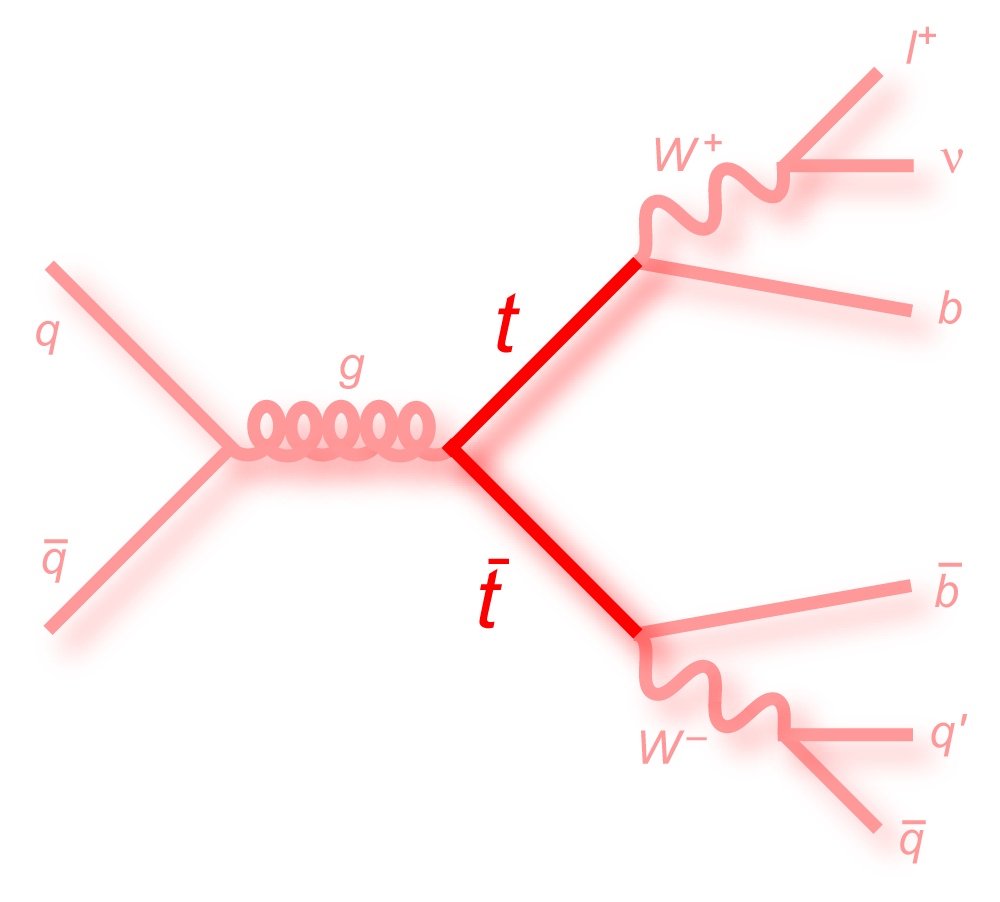
\includegraphics[width = 0.7\linewidth]{ttbar}
\caption{Feynman diagram of $t\bar{t}$ process}
\label{fig: ttbar_background}
\end{figure}

The other background considered for the analysis is the Drell-Yan process shown in Figure \ref{fig: DY_background}. The reason for this process to be considered as a background is the two leptons in its final state as well as the two jets coming from the initial state radiation jets. It can be seen that from the three backgrounds, Drell-Yan is the one that is the most similar to the heavy neutrino production, because the heavy neutrino process considered for this analysis also has two jets and two leptons in the final state. This is why the Drell-Yan background was expected to be the most difficult to separate from the signal of interest in the analysis.

\begin{figure}[H]
\centering
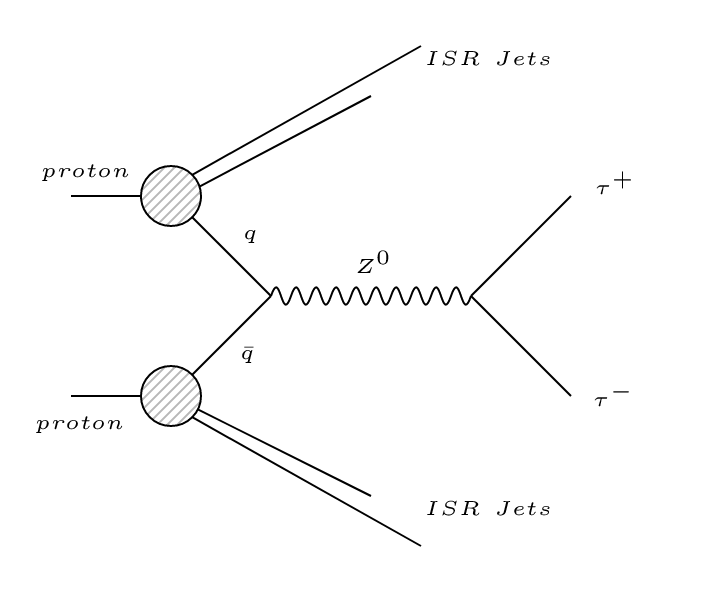
\includegraphics[width = 0.7\linewidth]{Drell-Yan}
\caption{Feynman diagram of Drell-Yan process}
\label{fig: DY_background}
\end{figure}